\documentclass[a4paper]{article}
\usepackage{amsmath}
\usepackage{amssymb}
\usepackage{xcolor}
\usepackage{amsthm}
\usepackage{dsfont}
\usepackage{graphicx}
\usepackage{hyperref}
\usepackage{datetime}
\usepackage{outlines}
\usepackage{float}

% code highlighting
\usepackage{minted}
\usepackage{xpatch}
\newminted[cminted]{python}{fontsize=\small}
\xpretocmd{\cminted}{\RecustomVerbatimEnvironment{Verbatim}{BVerbatim}{}}{}{}

% link coloring
%\hypersetup{
%    colorlinks,
%    linkcolor={red!80!black},
%    citecolor={green!60!black},
%    urlcolor={blue!80!black}
%}

% concatenation symbol (c.f. ++ in Haskell)
\newcommand\mdoubleplus{\mathbin{+\mkern-10mu+}}

% end of proof symbol
\newcommand{\newmarkedtheorem}[1]{%
  \newenvironment{#1}
    {\pushQED{\qed}\csname inner@#1\endcsname}
    {\popQED\csname endinner@#1\endcsname}%
  \newtheorem{inner@#1}%
}

\theoremstyle{definition}
%\newtheorem{eg}{Example}[section]
\newmarkedtheorem{eg}{Example}[section]
\newtheorem{observation}{Observation}[section]
\newtheorem{define}{Definition}[section]
\theoremstyle{plain}
\newtheorem{proposition}{Proposition}
\newtheorem{lemma}{Lemma}
\newtheorem{theorem}{Theorem}[section]
\newtheorem{assump}{Assumption}[section]
\newtheorem{remark}{Remark}[section]

\newdateformat{monthyeardate}{\monthname[\THEMONTH] \THEYEAR}

\author{Jeroen van Riel}
\date{\monthyeardate\today}
\title{}

\begin{document}

\subsection*{Vehicle dynamics}

In control theory, it is common to model motion dynamics of a system in terms of
a state vector $s(t) \in \mathbb{R}^{n}$ and a control input vector
$u(t) \in \mathbb{R}^{m}$, which result in a scalar position $y(t)$ via the
equations
\begin{subequations}\label{eq:control_equations}
\begin{align}
  \dot{s}(t) &= A s(t) + B u(t) , \\
  y(t) &= C s(t) .
\end{align}
\end{subequations}
%
Furthermore, the state and control trajectories are often restricted by imposing
linear constraints of the form
\begin{subequations}\label{eq:control_constraints}
\begin{align}
  G s(t) \leq b , \\
  F u(t) \leq d .
\end{align}
\end{subequations}
%
In the discussion that follows, each vehicle is modeled as a \textit{double integrator},
with $s(t) = (p(t), v(t))$, where $p(t)$ and $v(t)$ are the scalar position
along a predefined path and corresponding velocity, respectively. The three
matrices are chosen such that
\begin{align*}
  \dot{s}(t) &= \begin{pmatrix} 0 & 1 \\ 0 & 0 \end{pmatrix} s(t) + \begin{pmatrix} 0 \\ 1 \end{pmatrix} u(t), \\
  y(t) &= \begin{pmatrix} 1 & 0 \end{pmatrix} s(t),
\end{align*}
which may simply be rewritten as
\begin{align}
  \label{eq:motion_dynamics}
  \dot{p}(t) = v(t) , \quad
  \dot{v}(t) = u(t) , \quad
  y(t) = p(t) ,
\end{align}
where we recognize that the control input $u(t)$ corresponds directly to the
acceleration of the vehicle.


\subsection*{Intersection model}

Consider an intersection with $n$ incoming lanes. We define the index set
\begin{align*}
  \mathcal{N} = \{ (l, k) : k \in \{1, \dots, n_{l}\}, \; l \in \{1, \dots n\}\} ,
\end{align*}
where $n_{l}$ denotes the number of vehicles of lane $l$. To
further help with notation, given vehicle index $i = (r,s) \in \mathcal{N}$, we
define $l(i) = r$ and $k(i) = s$.

We assume that the position $p_{i}(t)$ of some vehicle $i \in \mathcal{N}$
corresponds to the physical front of the vehicle.
%
In order to model a safe distance between vehicles on the same lane, we require
that
\begin{align*}
  p_{i}(t) - p_{j}(t) \geq P_{i} ,
\end{align*}
for all $t$ and all pairs of indices $i, j \in \mathcal{N}$ such that
$l(i) = l(j), \; k(i) + 1 = k(j)$, with $P_{i} \geq 0$. Let $\mathcal{C}$ denote
the set of such ordered pairs of indices. Note that these constraints restrict
vehicles from overtaking each other.
%
Furthermore, in order to model collision avoidance, we say that a vehicle \textit{occupies the intersection}
whenever $p_{i}(t) \in [L, H_{i}] = \mathcal{E}_{i}$. The collision avoidance constraints are
given by
\begin{align*}
  (p_{i}(t), p_{j}(t)) \notin \mathcal{E}_{i} \times \mathcal{E}_{j},
\end{align*}
for all $t$ and for all pairs of indices $i, j \in \mathcal{N}$ with
$l(i) \neq l(j)$, which we collect in the set $\mathcal{D}$. Note that the length
of a vehicle can be modeled by choosing $H_{i}$ and $P_{i}$ appropriately.
%
Let $D_{i}(s_{i,0})$ denote the set of feasible trajectories
$x_{i}(t) = (s_{i}(t), u_{i}(t))$ given some initial state
$s_{i,0} = (p_{i}(0), v_{i}(0))$ and satisfying the vehicle dynamics given by
equations~\eqref{eq:motion_dynamics}. Given some performance criterion
$J(x_{i})$, the type of coordination problem we want to study is of the form
\begin{subequations}\label{eq:full_problem}
\begin{align}
  \min_{\mathbf{x}(t)} \quad & \sum_{i \in \mathcal{N}} J(x_{i}) \\
  \text{s.t.} \quad  & x_{i} \in D_{i}(s_{i,0}) , &\text{for all } i \in \mathcal{N} , \\
                & p_{i}(t) - p_{j}(t) \geq P_{i}, &\text{for all } (i,j) \in \mathcal{C} , \label{eq:follow_constraints} \\
                & (p_{i}(t), p_{j}(t))  \notin \mathcal{E}_{i} \times \mathcal{E}_{j} , &\text{for all } \{i,j\} \in \mathcal{D} \label{eq:collision_constraints} ,
\end{align}
\end{subequations}
where $\mathbf{x}(t) = [\, x_{i}(t) : i \in \mathcal{N} \,]$.

\subsection*{Direct transcription}

Optimization problem~\eqref{eq:full_problem} can be transcribed directly into a
non-convex mixed-integer linear program by discretization on a uniform time
grid. Let $K$ denote the number of discrete time steps and let $\Delta t$ denote
the time step size.
%
Using the forward Euler integration scheme, we have
\begin{subequations}
\begin{align*}
  p_{i}(t + \Delta t) = p_{i}(t) + v_{i}(t) \Delta t , \\
  v_{i}(t + \Delta t) = v_{i}(t) + u_{i}(t) \Delta t ,
\end{align*}
\end{subequations}
for each $t \in (0, \Delta t, \dots, K \Delta t)$.
The disjunctive constraints are formulated using the big-M technique by the constraints
\begin{subequations}
\begin{align*}
  p_{i}(t) \leq L + \delta_{i}(t) M , \\
  H - \gamma_{i}(t) M \leq p_{i}(t) , \\
  \delta_{i}(t) + \delta_{j}(t) + \gamma_{i}(t) + \gamma_{j}(t) \leq 3 ,
\end{align*}
\end{subequations}
where $\delta_{i}(t), \gamma_{i}(t) \in \{ 0, 1 \}$ for all $i \in \mathcal{N}$
and $M$ is a sufficiently large number.
%
Finally, the follow constraints can simply be added as
\begin{align*}
  p_{i}(t) - p_{j}(t) \geq P_{i} ,
\end{align*}
for each $t \in (0, \Delta t, \dots, K \Delta t)$ and each pair of consecutive
vehicles $(i, j) \in \mathcal{C}$.

For example, consider the objective functional
\begin{align}\label{eq:example_obj}
  J(x_{i}) = \int_{t=0}^{t_{f}} \left( {(v_{d} - v_{i}(t))}^{2} + {u_{i}(t)}^{2} \right) dt ,
\end{align}
where $v_{d}$ is some reference velocity and $t_{f}$ denotes the final time. For
example, see the optimal trajectories in
Figure~\ref{fig:direct_transcription_example}.

\begin{table}[H]
  \centering
\begin{tabular}{ c | c c c | c c }
  $i$  & (1,1) & (1,2) & (1,3) & (2,1) & (2,2) \\
  \hline
  $p_{i}$ & 15 & 10 &  0 & 10 &  0 \\
  $v_{i}$ & 10 & 10 & 10 & 10 & 10 \\
\end{tabular}
\caption{Example initial conditions for problem~\eqref{eq:full_problem}.}
\label{tab:hult_parameters}
\end{table}

\begin{figure}[H]
  \centering
  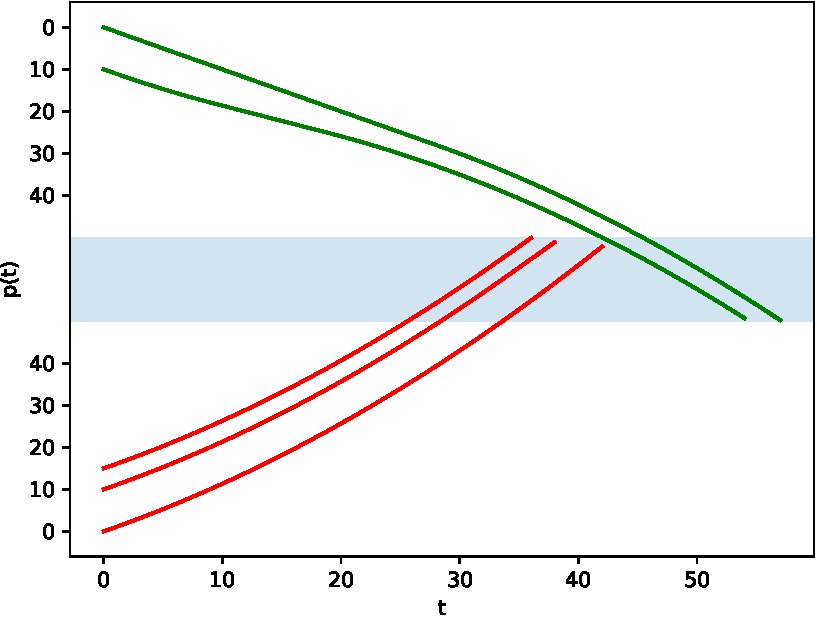
\includegraphics[width=0.8\textwidth]{figures/direct_transcription_example.pdf}
  \caption{Example of optimal trajectories obtained using the direct
    transcription method with
    $P_{i} = P = 5, \mathcal{E}_{i} = \mathcal{E} = [50, 70], v_{d} = 20, T=120, \Delta t = 0.1$
    and initial conditions as given in Table~\ref{tab:hult_parameters}. The
    y-axis is split such that each part corresponds to one of the two lanes and
    the trajectories are inverted accordingly and drawn with separate colors.
    The intersection area $\mathcal{E}$ is drawn as a shaded region. Whenever a
    vehicle has left the intersection, we stop drawing its trajectory for
    clarity.}
  \label{fig:direct_transcription_example}
\end{figure}


\subsection*{Crossing time criterion}

We start by considering a subclass of problems that allow us to almost ignore
the vehicle dynamics. As performance criterion, we consider the \textit{crossing
  time}
\begin{align}
  \label{eq:crossing_time_criterion}
  J(x_{i}) = \inf_{t} \{ t : p_{i}(t) = L \} .
\end{align}
Furthermore, we impose a maximum speed for every vehicle, so
\begin{align}
  \label{eq:max_speed_constraint}
  v_{i}(t) \leq v_\text{max} ,
\end{align}
for every $t$. We do not define any linear constraints on the control input, so
we assume \textit{instantaneous acceleration} is possible. For the purpose of
the following discussion, it is not necessary to rigorously define what we mean
by that. Define the \textit{earliest crossing time} of vehicle $i$ as
\begin{align*}
  r_{i} = &\inf_{x_{i}} J(x_{i}) \\
  &\text{s.t. } x_{i} \in D_{i}(s_{i,0})
\end{align*}
It is not hard to see that we must have $r_{i} = (L - p_{i}(0)) / v_\text{max}$.
%
Instead of optimizing in terms of trajectories $\mathbf{x}$, we consider first
finding a \textit{schedule} $y$ for the crossing times by solving
\begin{subequations}\label{eq:single_intersection_scheduling}
\begin{align}
  \min_{y} \quad & \sum_{i \in \mathcal{N}} y_{i} & \\
  \text{s.t.} \quad & r_{i} \leq y_{i} & \text{ for all } i \in \mathcal{N} , \\
  & y_{i} + \rho_{i} \leq y_{j} & \text{ for all } (i,j) \in \mathcal{C} , \label{eq:conjunctions} \\
  & y_{i} + \sigma_{i} \leq y_{j} \text{ or } y_{j} + \sigma_{j} \leq y_{i} & \text{ for all } \{i,j\} \in \mathcal{D} , \label{eq:disjunctions}
\end{align}
\end{subequations}
where $\rho_{i} = P_{i} / v_{\text{max}}$ and
$\sigma_{i} = (H_{i} - L) / v_{\text{max}}$. By using the well-known big-M
method,~\eqref{eq:single_intersection_scheduling} can be turned into a
mixed-integer program, for which solvers are readily available.
%
Finally, note that an instance $s$ of~\eqref{eq:single_intersection_scheduling}
is completely characterized by the tuple
\begin{align*}
  s = (\mathcal{N}, \rho, \sigma, r) .
\end{align*}


\begin{proposition}
  The coordination problem~\eqref{eq:full_problem} with performance criterion~\eqref{eq:crossing_time_criterion} and maximum speed
  constraints~\eqref{eq:max_speed_constraint} is equivalent with~\eqref{eq:single_intersection_scheduling}.
\end{proposition}
\begin{proof}
  We show that any feasible solution can be translated to a feasible solution to
  the other problem without changing the objective value.

  Consider a set of trajectories $\mathbf{x}(t)$. Consider some arbitrary
  vehicle $i \in \mathcal{N}$. It follows directly from the definition of $r_{i}$
  that we must have $J(x_{i}) \geq r_{i}$.
  %
  % conjunctions
  Consider a pair of consecutive vehicles $(i,j) \in \mathcal{C}$ on the same
  lane. For every $t \geq J(x_{i})$, trajectory $x_{i}$ must satisfy
  \begin{align*}
    p_{i}(t) \leq L + (t - J(x_{i})) v_{\text{max}}
  \end{align*}
  and by the constraint~\eqref{eq:follow_constraints}, trajectory $x_{j}$ must satisfy
  \begin{align*}
    p_{j}(t) \leq L + (t - J(x_{i})) v_{\text{max}} - P_{i} .
  \end{align*}
  Hence, we have $p_{j}(t) \leq L$ if and only if
  $t \leq J(x_{i}) + P_{i} / v_{\text{max}}$, which implies that
  $J(x_{j}) \geq J(x_{i}) + \rho_{i}$.
  %
  % disjunctions
  Consider a pair of vehicles $\{i, j\} \in \mathcal{D}$ on distinct lanes. By a
  similar reasoning, constraint~\eqref{eq:collision_constraints} implies that we have either
  $J(x_{i}) + \sigma_{i} \leq J(x_{j})$ or $J(x_{j}) + \sigma_{j} \leq J(x_{i})$.
  %
  %
  This shows that $y_{i} = J(x_{i})$ is a feasible schedule for~\eqref{eq:single_intersection_scheduling}.

  % schedule
  Now consider a feasible schedule $y_{i}$. For every $i \in \mathcal{N}$, we
  construct a trajectory $x_{i}$ such that $J(x_{i}) = y_{i}$ by setting
  $p_{i}(t) = p_{i}(0) + t (L - p_{i}(0)) / y_{i}$ for $0 \leq t < y_{i}$ and
  $p_{i}(t) = L + (t - y_{i}) v_{\text{max}}$ for $t \geq y_{i}$, so
  instantaneous acceleration is happening at $t=0$ and $t=y_{i}$.
\end{proof}


\subsection*{Ordering vehicles}

Instances and solutions of the crossing time optimization problem~\eqref{eq:single_intersection_scheduling} can be
represented very clearly by their \textit{disjunctive graph}, which we define next. Let
$(\mathcal{N}, \mathcal{C}, \mathcal{O})$ be a directed graph with nodes
$\mathcal{N}$ and the following two types of arcs. The \textit{conjunctive arcs} encode
the fixed order of vehicles driving on the same lane. For each
$(i,j) \in \mathcal{C}$, an arc from $i$ to $j$ means that vehicle $i$ reaches the
intersection before $j$ due to the follow constraints~\eqref{eq:conjunctions}. The \textit{disjunctive arcs}
are used to encode the decisions regarding the ordering of vehicles from
distinct lanes, corresponding to constraints~\eqref{eq:disjunctions}. For each pair
$\{i,j\} \in \mathcal{D}$, at most one of the arcs $(i,j)$ or $(j,i)$ can be present
in $\mathcal{O}$.

When $\mathcal{O} = \varnothing$, we say the disjunctive graph is
\textit{empty}. Each feasible schedule satisfies exactly one of the two
constraints in~\eqref{eq:disjunctions}. When $\mathcal{O}$ contains exactly one arc from every pair
of opposite disjunctive arcs, we say the disjunctive graph is \textit{complete}.
Note that such graph is acyclic and induces a unique topological ordering $\pi$
of its nodes. Conversely, every ordering $\pi$ of nodes $\mathcal{N}$ corresponds
to a unique complete disjunctive graph, which we denote by
$G(\pi) = (\mathcal{N}, \mathcal{C}, \mathcal{O}(\pi))$.

% edge weights
We define weights for every possible arc in a disjunctive graph. Every
conjunctive arc $(i, j) \in \mathcal{C}$ gets weight $w(i,j) = \rho_{i}$ and every
disjunctive arc $(i, j) \in \mathcal{O}$ gets weight $w(i,j) = \sigma_{i}$. Given
some vehicle ordering $\pi$, for every $j \in \mathcal{N}$, we recursively define
the lower bound
\begin{align}
  \text{LB}_\pi(j) = \max\{ r_{j}, \max_{i \in N^{-}_{\pi}(j)} \text{LB}_\pi(i) + w(i,j) \} ,
\end{align}
where $N^{-}_{\pi}(j)$ denotes the set of in-neighbors of node $j$ in $G(\pi)$.
Observe that this quantity is a lower bound on the crossing time, i.e., every
feasible schedule $y$ with ordering $\pi$ must satisfy $y_{i} \geq \text{LB}_\pi(i)$
for all $i \in \mathcal{N}$.
%
Next, we show that this lower bound is actually tight for optimal schedules,
which allows us to calculate the optimal crossing times $y^{*}$ once we know an
optimal ordering $\pi^{*}$ of vehicles.


\begin{proposition}\label{prop:active-schedule}
  If $y$ is an optimal schedule
  for~\eqref{eq:single_intersection_scheduling} with ordering $\pi$, then
  \begin{align}
    \label{eq:optimality}
    y_{i} = \text{\upshape LB}_{\pi}(i) \quad \text{ for all } i \in \mathcal{N} .
  \end{align}
\end{proposition}
\begin{proof}
  Suppose $y$ is an optimal schedule with ordering $\pi$. We write $\pi(k)$ for
  the $k$th element in the ordering, which is a permuation of $\mathcal{N}$.
  Consider the smallest $k \in \{1, \dots, |\mathcal{N}|\}$ such that vehicle
  $j = \pi(k)$ satisfies $y_{j} > \text{LB}_\pi(j)$. If no such $k$ exists, $y$
  already satisfies~\eqref{eq:optimality}. Otherwise, we construct a schedule
  $y'$ by setting $y'_{i} = y_{i}$ for every $i \in \mathcal{N}, i \neq j$ and
  $y'_{j} = \text{LB}_\pi(j)$.

  We now argue that $y'$ is stil a feasible schedule. Due to their direction, we
  only have to verify the inequalities
  in~\eqref{eq:single_intersection_scheduling} corresponding to incoming arcs
  $(i, j) = (\pi(r), \pi(k))$ with $r < k$. For these nodes $i$, we have
  $y_{i} = \text{LB}_\pi(i)$ by definition of $k$. From the definition of
  $\text{LB}$ then follows that
  \begin{align*}
    y'_{j} = \text{LB}_\pi(j) \geq \text{LB}_\pi(i) + w(i,j) = y'_{i} + w(i,j) ,
  \end{align*}
  which shows that all inequalities still hold.

  The new schedule has strictly better objective
  $\sum_{i \in \mathcal{N}} y'_{i} < \sum_{i \in \mathcal{N}} y_{i}$, which
  contradicts the assumption that $y$ is optimal.
\end{proof}


The previous result shows that we can concentrate on finding an optimal ordering
$\pi$. Under the condition that $\rho_{i} = \rho$ and $\sigma_{i} = \sigma > \rho$ for all
$i \in \mathcal{N}$, it turns out that some properties of an optimal ordering can
be immediately computed from the problem specification.
%
Before we present this rule, we first prove the following lemma that provides an
easier expression for calculating the lower bounds under these assumptions.

\begin{lemma}\label{lb_lemma}
  Let $\pi$ be some permutation of $\mathcal{N}$. Assume that
  $\sigma_{i} = \rho_{i} + s$, for every $i \in \mathcal{N}$, with $s > 0$.
  Consider a pair $i,j \in \mathcal{N}$ such that $i$ is the immediate predecessor
  of $j$ in $\pi$, so $\pi^{-1}(i) + 1 = \pi^{-1}(j)$, then
\begin{align}
  \label{eq:lb_lemma}
  \text{\upshape LB}_\pi(j) = \max \{ r_{j}, \text{\upshape LB}_\pi(i) + w(i, j) \} .
\end{align}
\end{lemma}
\begin{proof}
  Suppose $(i,j) \in \mathcal{C}$, see Figure~\ref{fig:lb_lemma},
  then the incoming disjunctive arcs of $j$ are
  $N^{-}_{\pi}(j) \setminus \{ i \} \subset N^{-}_{\pi}(i)$. Therefore, we have
  \begin{align*}
    \max_{v \in N^{-}_{\pi}(j) \setminus \{i\}} \text{LB}_\pi(v) + \sigma_{v} \leq \text{LB}_\pi(i) ,
  \end{align*}
  so that
      $\text{LB}_\pi(v) + w(v,j) \leq \text{LB}_\pi(i) + w(i,j)$
  for all $v \in N_{\pi}^{-}(j)$.

  Otherwise, we have $(i, j) \in \mathcal{O}(\pi)$.
  %
  Let $v \in \mathcal{N}$ such that $(v, j)$ is an arc.
  If $(v,j) \in \mathcal{C}$, then we have
  \begin{align*}
    \text{LB}_\pi(v) + w(v,j) =
    \text{LB}_\pi(v) + \rho_{v} \leq \text{LB}_\pi(v) + \sigma_{v} + \sigma_{i} \leq \text{LB}_\pi(i) + w(i,j) ,
  \end{align*}
  where the second inequality follows from $(v,i) \in \mathcal{O}(\pi)$.
  %
  If $(v, j) \in \mathcal{O}(\pi)$ with $l(v) \neq l(i)$, then $(v,i) \in \mathcal{O}(\pi)$, so
  \begin{align*}
    \text{LB}_\pi(v) + w(v, j) = \text{LB}_\pi(v) + w(v, i) \leq \text{LB}_\pi(i) \leq \text{LB}_\pi(i) + w(i,j) .
  \end{align*}
  If $(v, j) \in \mathcal{O}(\pi)$ with $l(v) = l(i)$, then there is a path of conjunctive arcs between $v$ and
  $i$, so we must have $\text{LB}_\pi(v) + \rho_{v} \leq \text{LB}_\pi(i)$.
  Furthermore, from $w(v,j) = \sigma_{v} = \rho_{v} + s$ follows that
  \begin{align*}
    \text{LB}_\pi(v) + w(v,j) = \text{LB}_\pi(v) + \rho_{v} + s \leq \text{LB}_\pi(i) + s \leq \text{LB}_\pi(i) + w(i, j) .
  \end{align*}

  To conclude, we have shown that
  $\text{LB}_\pi(v) + w(v,j) \leq \text{LB}_\pi(i) + w(i,j)$ for any
  $v \in N^{-}_{\pi}(j)$, from which statement~\eqref{eq:lb_lemma} follows.
\end{proof}

\begin{figure}
  \centering
  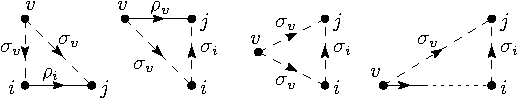
\includegraphics[width=0.9\textwidth]{figures/lower-bound-lemma.pdf}
  \caption{Sketch of the four cases distinguished in the proof of
    Lemma~\ref{lb_lemma}. Arc weights are given and disjunctive arcs
    $\mathcal{O}(\pi)$ are drawn with a dashed line.}\label{fig:lb_lemma}
\end{figure}


\begin{proposition}\label{prop:exhaustive}
  Consider an instance of~\eqref{eq:single_intersection_scheduling} with $\rho_{i} = \rho$ and $\sigma_{i} = \sigma > \rho$ for all
  $i \in \mathcal{N}$. Suppose $y$ is an optimal schedule with
  $y_{i^{*}} + \rho \geq r_{j^{*}}$, for some $(i^{*},j^{*}) \in \mathcal{C}$, then
  $j^{*}$ follows immediately after $i^{*}$, so $y_{i^{*}} + \rho = y_{j^{*}}$.
\end{proposition}
\begin{proof}
  Suppose the ordering $\pi$ of $y$ is such that
  $\pi^{-1}(i^{*}) + 1 < \pi^{-1}(j^{*})$.
  %
  Let $\mathcal{I}(i,j) = \{ i, \pi(\pi^{-1}(i) + 1), \dots, j \}$ be the set of
  vehicles between $i$ and $j$.
  %
  Let $f = \pi(1)$ and $e = \pi(|\mathcal{N}|)$ be the first and last vehicles,
  respectively, and set $u = \pi^{-1}(i^{*}) + 1$ and $v = \pi^{-1}(j^{*}) - 1$, see also Figure~\ref{fig:platoon-preservation-diagram}.
  Construct new ordering $\pi'$ by moving vehicle $j^{*}$ forward
  by $|\mathcal{I}(u,v)|$ places and let $y'$ denote the corresponding schedule.
  %
  We have $y_{i} = y'_{i}$ for all $i \in \mathcal{I}(f, i^{*})$, so these do not
  contribute to any difference in the objective.
  %
  Using Proposition~\ref{prop:active-schedule} and Lemma~\ref{lb_lemma}, we compute
  \begin{align*}
    y'_{j^{*}} &= \max \{ r_{j^{*}}, y_{i^{*}} + \rho \} = y_{i^{*}} + \rho , \\
    y_{u} &= \max \{ r_{u}, y_{i^{*}} + \sigma \} , \\
    y'_{u} &= \max \{ r_{u}, y_{i^{*}} + \rho + \sigma \} ,
  \end{align*}
  where we used that $y_{i^{*}} + \rho \geq r_{j^{*}}$ by assumption.
  %
  Note that we have
  $y_{i^{*}} + \sigma + (|\mathcal{I}(u,v)| - 1) \rho \leq y_{v}$, regardless of the
  type of arcs between consecutive vehicles in $\mathcal{I}(u,v)$. Therefore,
  \begin{align*}
    y_{j^{*}} - y'_{j^{*}} \geq y_{v} + \sigma - y_{i^{*}} - \rho \geq 2 \sigma + (|\mathcal{I}(u,v)| - 2) \rho .
  \end{align*}

  We now show that $y'_{k} \geq y_{k}$ and $y'_{k} - y'_{j^{*}} \leq y_{k} - y_{i^{*}}$ for every $k \in \mathcal{I}(u,v)$.
  For $k = u$, it is clear that $y'_{u} \geq y_{u}$ and
  \begin{align*}
    y'_{u} - y'_{j^{*}} = \max \{ r_{u} - (y_{i^{*}} + \rho), \sigma \} \leq \max \{ r_{u} - y_{i^{*}}, \sigma \} = y_{u} - y_{i^{*}}.
  \end{align*}
  Now proceed by induction and let $x$ be the immediate predecessor of $k$ for
  which the inequalities hold, then
  \begin{align*}
    y'_{k} = \max \{ r_{k}, y'_{x} + w(x,k) \} \geq \max \{ r_{k}, y_{x} + w(x,k) \} = y_{k}
  \end{align*}
  and the second inequality follows from
  %\begin{align*}
  %  y'_{k} - y'_{x} = \max \{ r_{k} - y'_{x}, w(x,k) \} &\leq \max \{ r_{k} - y_{x}, w(x,k)\} = y_{k} - y_{x}
  %\end{align*}
  %implies that
  %\begin{align*}
  %  y'_{k} - y'_{j^{*}} = (y'_{k} - y'_{x}) + (y'_{x} - y'_{j^{*}}) \leq (y_{k} - y_{x}) + (y_{x} - y_{i^{*}}) = y_{k} - y_{i^{*}} .
  %\end{align*}
  %
  \begin{align*}
    (y'_{k} - y'_{x}) + (y'_{x} - y'_{j^{*}}) &= \max \{ r_{k} - y'_{x}, w(x,k) \} + (y'_{x} - y'_{j^{*}}) \\
                                             &\leq \max \{ r_{k} - y_{x}, w(x,k) \} + (y_{x} - y_{i^{*}}) \\
                                             &= (y_{k} - y_{x}) + (y_{x} - y_{i^{*}}) .
  \end{align*}

  Let $l$ denote the immediate successor of $j^{*}$, if there is one. Regardless of
  whether $j^{*}$ and $l$ are in the same lane, we have
  $y_{j^{*}} + \rho \leq y_{l}$. We derive
  \begin{align*}
    y'_{v} = y'_{v} - y'_{j^{*}} + y'_{j^{*}} \leq y_{v} - y_{i^{*}} + y'_{j^{*}} = y_{v} + \rho \leq y_{j^{*}} - \sigma + \rho ,
  \end{align*}
  from which follows that $y'_{v} + \sigma \leq y_{l}$,
  %\begin{align*}
  %  y'_{v} + \sigma = (y'_{v} - y'_{j^{*}}) + y'_{j^{*}} + \sigma \leq y_{v} - y_{i^{*}} + y'_{j^{*}} + \sigma = y_{v} + \rho + \sigma \leq y_{j^{*}} + \rho \leq y_{l} ,
  %\end{align*}
  which means that $y_{i} \geq y'_{i}$ for $i \in \mathcal{I}(l, e)$.

  We can now compare the objectives by putting everything together
  \begin{align*}
    \sum_{i \in \mathcal{N}} y_{i} - y'_{i} &=  y_{j^{*}} - y'_{j^{*}} + \sum_{i \in \mathcal{I}(u, v)} y_{i} - y'_{i} + \sum_{i \in \mathcal{I}(l, e)} y_{i} - y'_{i} \\
    &\geq 2 \sigma + (|\mathcal{I}(u,v)| - 2) \rho + \sum_{k \in \mathcal{I}(u,v)} (y_{k} - y_{i^{*}}) - (y'_{k} - y'_{j^{*}}) \\ & \hspace{12em} - |\mathcal{I}(u,v)| (y'_{j^{*}} - y_{i^{*}}) \\
    &\geq 2 \sigma - 2 \rho > 0
  \end{align*}
  which contradicts the assumption that $y$ and $\pi$ were optimal.
  %
  Finally, from Proposition~\ref{prop:active-schedule} and Lemma~\ref{lb_lemma}
  follows that $y_{i^{*}} + \rho = y_{j^{*}}$.
\end{proof}

\begin{figure}
  \centering
  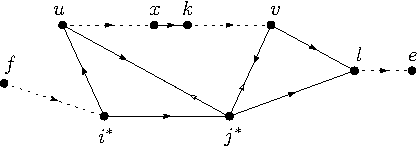
\includegraphics[width=0.8\textwidth]{figures/platoon-preservation-proof-diagram.pdf}
  \caption{Sketch of the nodes and most important arcs used in the proof of
    Proposition~\ref{prop:exhaustive}. Dashed arcs represent chains of
    unspecified length. The two open arrows indicate the new direction of their
    arc under ordering $\pi'$.}\label{fig:platoon-preservation-diagram}
\end{figure}


\subsection*{Partial ordering}

% constructive scheduling
Finding an optimal schedule by solving the mixed-integer linear program boils
down to systematically evaluating all different schedules. This method does not
scale well to larger instances, so we are interested in good heuristics. A
common approach in the scheduling literature is to incrementally construct a
schedule by fixing one job starting time (vehicle crossing time) at each step.
%
We will consider incrementally constructing a vehicle ordering. Therefore, we
define partial ordering $\pi$ to be a \textit{partial permutation} of
$\mathcal{N}$, which is a sequence of elements from some subset
$\mathcal{N}(\pi) \subset \mathcal{N}$.
%
Let $\pi$ be a partial ordering of length $n$ and let
$i \notin \mathcal{N}(\pi)$, then we use $\pi' = \pi \mdoubleplus i$ to denote
the concatenation of sequence $\pi$ with $i$, so $\pi'_{1:n} = \pi_{1:n}$ and
$\pi'_{n+1} = i$. Furthermore, recursively define the concatenation of two
sequences by
$\pi \mdoubleplus \pi' = ( \pi \mdoubleplus \pi'_{1} ) \mdoubleplus \pi'_{2:m}$,
where $m$ is the length of $\pi'$.

For each partial ordering $\pi$, the corresponding disjunctive graph $G(\pi)$ is
incomplete, meaning that some of the disjunctive arcs have not yet been added.
Nevertheless, observe that $\text{LB}_{\pi}(i)$ is still defined for every
$i \in \mathcal{N}$.
%
Now consider the following rule for partial orderings, which is a generalization
of Proposition~\ref{prop:exhaustive}, because
$\text{LB}_{\pi'}(i^{*}) = r_{i^{*}}$ for the empty ordering
$\pi = \varnothing$.

\begin{proposition}\label{prop:exhaustive_partial}
  % same assumptions as in prop:exhaustive
  Consider an instance of~\eqref{eq:single_intersection_scheduling} with
  $\rho_{i} = \rho$ and $\sigma_{i} = \sigma > \rho$ for all
  $i \in \mathcal{N}$.
  %
  Let ${\pi}$ be a partial ordering of length $n$. If ${\pi}$ is such that
  $\text{LB}_{{\pi}}(i^{*}) + \rho_{i^{*}} \geq r_{j^{*}}$ for some
  $(i^{*},j^{*}) \in \mathcal{C}$ with $i^{*}, j^{*} \notin {\pi}$, then $j^{*}$ follows
  immediately after $i^{*}$ in any complete optimal ordering ${\pi} \mdoubleplus \pi'$.
\end{proposition}
\begin{proof}
  Consider a new problem instance $s'$ on the unscheduled vehicles
  $\mathcal{N}' = \mathcal{N} \setminus \mathcal{N}({\pi})$, with
  $r'_{i} = \text{LB}_{{\pi}}(i)$ for all $i \in \mathcal{N}'$.
  It follows from Proposition~\ref{prop:exhaustive} that $j^{*}$ follows $i^{*}$
  immediately in any optimal ordering $\pi'$ of the remaining vehicles.
\end{proof}


\newpage

\subsection*{Lane ordering}

% automaton
Observe that ordering vehicles is equivalent to ordering the lanes, due to the
conjunctive constraints. We propose a method based on repeatedly choosing the
next lane. This may be modeled as a deterministic finite-state automaton, where
the set of lane indices acts as the input alphabet $\Sigma = \{ 1, \dots, n \}$,
where $n$ denotes the number of lanes. Let $S$ denote the state space and let
$\delta: S \times \Sigma \rightarrow S$ denote the state-transition function.

% states
Let $s$ denote an instance of~\eqref{eq:single_intersection_scheduling}. We
consider $s$ to be a fixed part of the state, so it does not change with state
transitions.
The other part of the state is the current partial ordering $\pi$.
% transitions
The transitions of the automaton are very simple. Let $(s, \pi) \in S$ denote
the current state and let $l \in \Sigma$ denote the next symbol. Let
$i \in \mathcal{N} \setminus \mathcal{N}(\pi)$ denote the next unscheduled vehicle on lane $l$,
then the system transitions to $(s, \pi \mdoubleplus i)$. If no such vehicle exists, the
transition is undefined. Observe that some lane sequence $\eta$ is valid
whenever it is of length
\begin{align*}
  N = \sum_{l \in \Sigma} n_{l}
\end{align*}
and contains precisely $n_l = |\{ i \in \mathcal{N} : l(i) = l \}|$ occurrences
of $l$, for each $l \in \Sigma$.
%
Let $\delta(s, \eta)$ denote the state
that we obtain after applying sequence $\eta$ to the automaton with initial
state $s_{0} = (s, \varnothing)$, which generalizes the single step transition function by
recursively defining
\begin{align*}
  \delta(s, \eta_{1:t}) = \delta(\delta(s, \eta_{1:t-1}), \eta_{t}) .
\end{align*}


\subsection*{Behavioral cloning}

% policy
It is now clear that task of finding an optimal schedule has been reduced to
finding an optimal lane sequence.
%
Therefore, our goal is now to find a mapping from problem instances to optimal lane sequences.
This mapping is of course very complex, so our aim is to find a good approximation.
%
Instead of formulating a direct mapping, we model the conditional distribution
$p_{\theta}(\eta | s)$ of the optimal lane sequence given a problem instance $s$
and we factorize it as
%
\begin{align*}
  p_{\theta} (\eta \, | \, s) = \prod_{t=1}^{N} p_{\theta}(\eta_{t} \, | \; \delta(s, \eta_{1:t-1})) ,
\end{align*}
%
where $\theta$ denotes the model parameters. We aim to learn this conditional
distribution from a set of instances with corresponding optimal schedules.
%
Given problem instance $s$, let $y_{\eta}(s)$ denote the schedule obtained from
lane order $\eta$. We first compute an optimal schedule $y^{*}(s)$. Next, we
compute $\eta$ such that $y^{*}(s) = y_{\eta}(s)$ to obtain the corresponding
trajectory of states $s_{t} = \delta(s, \eta_{1:t})$. The resulting set of pairs
$(s_{t}, \eta_{t})$ can be used to learn $p_{\theta}$ in a supervised fashion by
treating it as a classification task.

% inference
We employ \textit{greedy inference} as follows. The model $p_{\theta}$ provides
a distribution over the lanes. We ignore the lanes that have no unscheduled
vehicles anymore and take the argmax of the remaining probabilities. We will
denote the corresponding complete schedule by $\hat{y}_{\theta}(s)$.

\subsection*{Parameterization}

We will now discuss two ways of parameterizing the model. In both cases, we
first derive, for every $l \in \Sigma$, a \textit{lane embedding} $h_{l}(s_{t})$
based on the current nonterminal state $s_{t} = (s, \pi_{t})$ of the automaton.
We then apply the following trick, which we call \textit{lane cycling}.
Let $\eta_{t}$

These embeddings are then mapped to a probability distribution
\begin{align*}
  p_{\theta}(\eta_{t+1} | s_{t}) = f_{\theta}(h(s_{t})) ,
\end{align*}
where $f_{\theta}$ is a fully connected neural network.


\subsubsection*{Padded embedding}
%
Let $k_{\pi}(l)$ denote the first unscheduled vehicle in lane $l$ under the partial schedule $\pi_{t}$.
Denote the smallest lower bound of unscheduled vehicles as
\begin{align*}
  T_{\pi} = \min_{i \in \mathcal{N} \setminus \mathcal{N}(\pi)} \text{LB}_{\pi}(i) .
\end{align*}
Let the \textit{horizon} of lane $l$ be defined as
\begin{align*}
  h_{l}(s_{t}) = ( \text{LB}_{\pi_{t}}(k_{\pi_{t}}(l)) - T_{\pi_{t}}, \dots, \text{LB}_{\pi_{t}}(n_{l}) - T_{\pi_{t}} ) .
\end{align*}

Observe that horizons can be of arbitrary dimension. Therefore, we restrict each
horizon to a fixed length $\Gamma$ and use zero padding. More precisely, given a
sequence $x = (x_{1}, \dots, x_{n})$ of length $n$, define the padding
operator
\begin{align*}
  \text{pad}(x, \Gamma) = \begin{cases}
                            (x_{1}, \dots, x_{\Gamma}) &\text{ if } \Gamma \leq n,  \\
                            (x_{1}, \dots, x_{n}) \mdoubleplus (\Gamma - n) * (0) &\text{ otherwise, }
                            \end{cases}
\end{align*}
where we use the notation $n * (0)$ to mean a sequence of $n$ zeros. The full
observation is now given by
\begin{align*}
  h(s_{t}) = (\text{pad}(h_{1}(s_{t}), \Gamma), \dots, \text{pad}(h_{|\Sigma|}(s_{t}), \Gamma)) .
\end{align*}
%

\subsubsection*{Recurrent embedding}

To avoid the zero padding operation, which can be problematic for states that
are almost done, we can employ a recurrent architecture that is agnostic to the
number of remaining unscheduled vehicles.

\subsection*{Experiments}

We consider an intersection with $2$ approaching lanes.
Instances are generated by sampling $g_{i}$ and $\rho_{i}$ and setting
\begin{align*}
  r_{i} = \sum_{k=1}^{k(i)} g_{i} + \sum_{k=1}^{k(i) - 1} \rho_{i} ,
\end{align*}
for each $i \in \mathcal{N}$. Let $\mathcal{X}$ denote the
training data, consisting of pairs of $(s_{t}, \eta_{t})$ as obtained from exact
solutions as explained above.


%
We interpret $p_{\theta}(s_{t})$ as the probability of choosing lane $1$.
We use the binary cross entropy loss
\begin{align*}
  - \frac{1}{|\mathcal{X}|} \sum_{(s_{t}, \eta_{t}) \in \mathcal{X}} \mathds{1}\{\eta_{t} = 1\} \log(p_{\theta}(s_{t})) + \mathds{1}\{\eta_{t} = 2\} \log(1 - p_{\theta}(s_{t})) ,
\end{align*}
where we use $\mathds{1}(\cdot)$ to denote the indicator function.
We use learning rate $10^{-3}$ and the Adam optimizer.
%
Let $\mathcal{Y}$ denote a set of test instances.
Let $\text{obj}(y)$ denote the objective of schedule $y$, then
we report on the average approximation ratio defined as
\begin{align*}
\hat{y}_{\theta} / y^{*} = \frac{1}{|\mathcal{Y}|} \sum_{s \in \mathcal{Y}} \text{obj}(\hat{y}_{\theta}(s)) \; / \; \text{obj}(y^{*}(s)) .
\end{align*}

We are particularly interested in the ability of the model to generalize to
instances with more vehicles, because this is where the MILP solving time
begins to become prohibitive.

%\begin{table}
%  \centering
%  \begin{tabular}{c c c}
%    $g_{i}$ & $\rho_{i}$ & $\hat{y}_{\theta} / y^{*}$ \\
%    \hline
%    $\text{Uni}(0, 4)$ & $ \text{Uni}(1,4) $ & 1 \\
%    $\text{Exp}(4)$ & $ \text{Uni}(1,4) $ & 1
%  \end{tabular}
%  \caption{Results (placeholder).}
%\end{table}

\subsection*{Discussion}

It might be insightful to compare the model probability of the computed greedy
schedule to the model probability of the optimal solution computed using
mixed-integer linear programming. This provides us an indication of model fit
and whether greedy inference is good enough or methods like beam search might be
necessary.

It might be interesting to analyze the feature attribution of the neural network
using a method like Integrated Gradients.

%\newpage
%\subsection*{Reinforcement learning}
%
%If we define rewards for the transitions
%\begin{align*}
%  r : S \times \Sigma \rightarrow \mathbb{R} ,
%\end{align*}
%then we obtain a deterministic Markov Decision Process.


%\section*{Related Literature}
%
%Discuss the paper ``Machine Learning for Combinatorial Optimization: a
%Methodological Tour d'Horizon''~\cite{bengioMachineLearningCombinatorial2020}.
%%
%Learning through behavioral cloning.
%Learning through reinforcement learning, requires the definition of rewards.
%Machine learning for end-to-end algorithm or in parts of branch-and-bound algorithms.

\newpage

\section*{Implementation details}

Recall that instances of
problem~\eqref{eq:single_intersection_scheduling} are completely characterized
by
\begin{align*}
  s = (\mathcal{N}, \rho, \sigma, r) .
\end{align*}
Throughout the code, it is assumed that
\begin{align*}
  \sigma_{i} = \rho_{i} + s ,
\end{align*}
because this allows us to use the result from Lemma~\ref{lb_lemma}.
Therefore, instances are represented by specifying earliest crossing time
$r_{i}$, length $\rho_{i}$ and \textit{switch-over} time $s$.
We will refer to earliest crossing time as the \textit{release time} of the vehicle.
Instances are represented in the code as basic dictionaries of the form
\begin{figure}[H]
\centering
\begin{cminted}
instance = {
    'release': [[1, 2, 4], [1, 2]],
    'length':  [[1, 2, 1], [1, 1]],
    'switch':  2
}
\end{cminted}
\end{figure}
%
\noindent
Instances and (partial) schedules can be visualized using
\texttt{util.plot\_schedule()}. For example, instance above together with the optimal
solution is given in the following figure.
\begin{figure}[H]
\centering
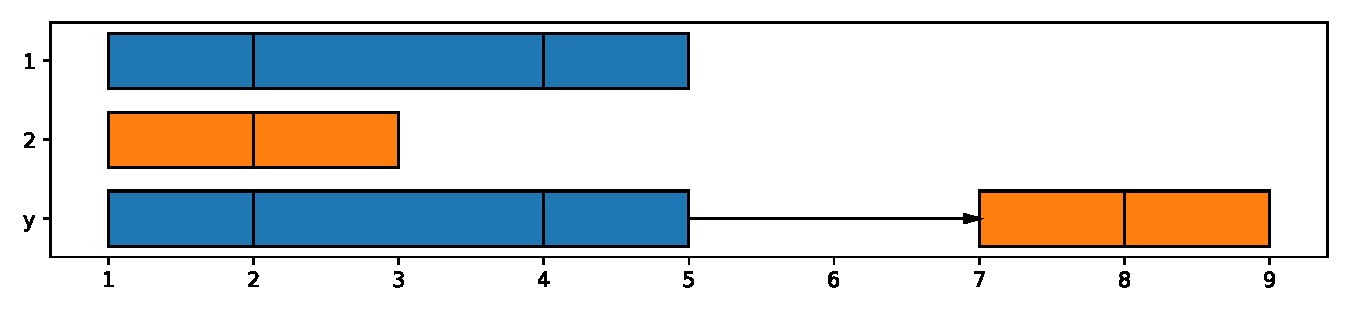
\includegraphics[width=0.9\textwidth]{figures/example_schedule.pdf}
\end{figure}
\noindent
Each vehicle is drawn as a rectangle, whose width represents $\rho_{i}$. The color
of each rectangle corresponds to its lane. The first two rows of the figure
visualize the instance specification and the last row visualizes the optimal
schedule $y$. The arrow visualizes the switch-over time $s$.

The automaton keeps track of $\text{LB}_{\pi}(i)$ for each node $i$, given the
current partial ordering. It provides these values as basic observations. We
transform these into the desired observations for training our heuristic. The method
\begin{figure}[H]
\centering
\begin{cminted}
  Automaton.exhaustive(lane)
\end{cminted}
\end{figure}
%
\noindent
returns whether the rule of
Proposition~\ref{prop:exhaustive_partial} applies to the given lane.



\newpage

\subsection*{Bibliographical notes}

The disjunctive graph is a common formalism used for job shop scheduling
problems (see Chapter 7 of~\cite{pinedoSchedulingTheoryAlgorithms2016}), to
which our crossing time scheduling problem is related. Furthermore, in
scheduling theory terminology, the result of
Proposition~\ref{prop:active-schedule} says that optimal schedules are
necessarily \textit{semi-active schedules}, see Definition 2.3.5
in~\cite{pinedoSchedulingTheoryAlgorithms2016}.
%
The rule for optimal orderings (Proposition~\ref{prop:exhaustive}) is equivalent
to the \textit{Platoon Preservation Theorem} of
Limpens~\cite{limpensOnlinePlatoonForming2023}.

Machine learning has been used extensively to solve combinatorial problems, see
for example the seminal paper~\cite{belloNeuralCombinatorialOptimization2017} and surveys~\cite{bengioMachineLearningCombinatorial2020,mazyavkinaReinforcementLearningCombinatorial2020}.

\bibliography{references}
\bibliographystyle{ieeetr}


\end{document}

% to enable the minted package
% Local Variables:
% TeX-command-extra-options: "-shell-escape"
% End:
